\documentclass[11pt]{article}
\DeclareUnicodeCharacter{3000}{}
% Libraries.
\usepackage{amsmath}
\usepackage{amssymb}
\usepackage{pgfplots}
\usepackage{graphicx}
\usepackage{enumitem}
\usepackage{hyperref}
\usepackage{fancyhdr}
\usepackage{perpage}
\usepackage{float}
\usepackage{esint}
\usepackage[margin=1.5cm]{geometry}

% Property settings.
\MakePerPage{footnote}
\pagestyle{headings}

% Commands
\newcommand{\ti}[1]{\textit{#1}}
\newcommand{\tb}[1]{\textbf{#1}}
\newcommand{\mb}[1]{\mathbb{#1}}
\newcommand{\mc}[1]{\mathcal{#1}}
\newcommand{\bx}[0]{\mathbf{x}}
\newcommand{\bv}[0]{\mathbf{v}}
\newcommand{\bw}[0]{\mathbf{w}}
\newcommand{\real}[0]{\mathbb{R}}
\newcommand{\under}[1]{\underline{#1}}
\newcommand{\proof}[0]{\textit{\underline{proof:} }}
\newcommand{\func}[3]{\tb{#1}: {#2} \rightarrow {#3} }
\newcommand{\vx}[0]{\tb{x}}
\newcommand{\vy}[0]{\tb{y}}
\newcommand{\vz}[0]{\tb{z}}
\newcommand{\vo}[0]{\tb{0}}
\newcommand{\va}[0]{\tb{a}}
\newcommand{\vb}[0]{\tb{b}}
\newcommand{\vc}[0]{\tb{c}}
\newcommand{\ve}[0]{\tb{e}}
\newcommand{\vm}[0]{\tb{m}}
\newcommand{\vh}[0]{\tb{h}}
\newcommand{\vf}[0]{\tb{F}}
\newcommand{\vi}[0]{\tb{i}}
\newcommand{\vj}[0]{\tb{j}}
\newcommand{\vk}[0]{\tb{k}}
\newcommand{\vg}[0]{\tb{G}}
\newcommand{\vn}[0]{\tb{n}}
\newcommand{\vu}[0]{\tb{u}}
\newcommand{\vv}[0]{\tb{v}}
\newcommand{\vL}[0]{\tb{L}}
\newcommand{\ff}[0]{\tb{f}}
\newcommand{\fg}[0]{\tb{g}}
\newcommand{\p}[0]{\partial}
\newcommand{\qed}[0]{$\hfill\blacksquare$}
\newcommand{\qerat}{\tag*{$\blacksquare$}}
\newcommand{\lima}{\underset{\vx \rightarrow \va}{\lim}}
\usepackage{amsmath}% http://ctan.org/pkg/amsmath
\newcommand{\notimplies}{%
  \mathrel{{\ooalign{\hidewidth$\not\phantom{=}$\hidewidth\cr$\implies$}}}}
\newcommand{\q}[0]{\textcolor{red}{???}}
\newcommand{\tspace}[0]{T_{x_0}}
\newcommand{\tanspace}[0]{T_{x_0}M}
% Attr.
\title{APM462 \\ Lecture Notes}
\author{Yuchen Wang}
\date{\today}

\begin{document}
    \maketitle
    \tableofcontents
    \newpage
    
\section{Matrix Calculus}
\paragraph{Row v.s. Column Vector}
Our default rule is that every vector is a column vector unless explicitly stated otherwise. \\
This is also known as the \under{numerator layout}. \\
\under{Special case}: For $f: \real^n \rightarrow \real$, $Df$ is a $ 1 \times n$ matrix or row vector.

\subsection{Matrix Multiplication}
\paragraph{Definition 1.1.1}
Let A be $m \times n$, and B be $n \times p$, and let the product AB be
$$C = AB$$
then $C$ is a $m \times p$ matrix, with element $(i,j)$ given by
$$c_{ij} = \sum_{k=1}^n a_{ik}b_{kj}$$
for all $i = 1, 2, \hdots, m, j = 1,2,\hdots,p$.
\paragraph{Proposition 1.1.2}
Let $A$ be $m \times n$, and $x$ be $n \times 1$, then the typical element of the product
$$ z = Ax$$
is given by
$$z_i = \sum_{k=1}^n a_{ik}x_k$$
for all $i= 1,2,\hdots,m$.\\
Similarly, let $y$ be $m \times 1$, then the typical element of the product
$$z^T = y^TA$$
is given by
$$ z_i^T = \sum_{k=1}^n a_{ki}y_k$$
for all $i = 1, 2,\hdots, n$.  \\
Finally, the scalar resulting from the product
$$\alpha = y^T A x$$
is given by
$$\alpha = \sum_{j=1}^m\sum_{k=1}^n a_{jk}y_i x_k$$

\subsection{Partitioned Matrices}
\paragraph{Proposition 1.2.1}
Let $A$ be a square, nonsingular matrix of order $m$. Partition A as
$$ A = \begin{bmatrix}
	A_{11} & A_{12} \\
	A_{21} & A_{22}
\end{bmatrix}
$$
so that $A_{11}$ and $A_{22}$ are invertible. \\
Then
$$ A^{-1} = \begin{bmatrix}
	(A_{11} - A_{12}A_{22}^{-1}A_{21})^{-1} & -A_{11}^{-1}A_{12}(A_{22} - A_{21}A_{11}^{-1}A_{12})^{-1} \\
	-A_{22}^{-1}A_{21}(A_{11} - A_{12}A_{22}^{-1}A_{21})^{-1} & (A_{22} - A_{21}A_{11}^{-1}A_{12})^{-1}
\end{bmatrix}$$
\proof \\
Direct multiplication of the proposed $A^{-1}$ and $A$ yields
$$A^{-1}A = I$$ \qed

\subsection{Matrix Differentiation}
\paragraph{Proposition 1.3.1}
$$\frac{\partial A}{\partial x} = \frac{\partial A^T}{\partial x}$$
\paragraph{Proposition 1.3.2}
Let $$y = Ax$$
where $y$ is $m\times 1$, $x$ is $n \times 1$, A is $m \times n$, and $A$ does not depend on $x$. Suppose that $x$ is a function of the vector $z$, while $A$ is independent of $z$. Then
$$\frac{\partial y }{\partial z} = A \frac{\partial x}{\partial z}$$

\paragraph{Proposition 1.3.3}
Let the \textcolor{red}{scalar} $\alpha$ be defined by
$$\alpha = y^T Ax$$
where $y$ is $m \times 1$, $x$ is $n \times 1$, $A$ is $m \times n$, and $A$ is independent of $x$ and $y$, then
$$\frac{\partial \alpha}{\partial x} = y^TA$$
and 
$$\frac{\partial \alpha}{\partial y} = x^TA^T$$

\paragraph{Proposition 1.3.4}
For the special case where the \textcolor{red}{scalar} $\alpha$ is given by the quadratic form
$$\alpha = x^TAx$$
where $x$ is $n \times 1$, $A$ is $n \times n$, and $A$ does not depend on $x$, then
$$\frac{\partial \alpha}{\partial x} = x^T (A + A^T)$$
\proof \\
By definition
$$\alpha = \sum_{j=1}^n \sum_{i=1}^n a_{ij}x_ix_j$$
Differentiating with respect to the $k$th element of $x$ we have
$$\frac{\partial \alpha}{\partial x_k} = \sum_{j=1}^n a_{kj}x_J + \sum_{i=1}^n a_{ik}x_i$$
for all $k = 1,2, \hdots, n$, and consequently,
$$\frac{\partial \alpha}{\partial x} = x^TA^T + x^TA = x^T(A^T + A)$$ \qed

\paragraph{Proposition 1.3.4}
For the special case where \textcolor{red}{$A$ is a symmetric matrix} and
$$\alpha = x^TAx$$
where $x$ is $n \times 1$, $A$ is $n \times n$, and $A$ does not depend on $x$, then
$$\frac{\partial \alpha}{\partial x} = 2x^TA$$

\paragraph{Proposition 1.3.5}
Let the \textcolor{red}{scalar} $\alpha$ be defined by
$$\alpha = y^Tx$$
where $y$ is $n \times 1$, $x$ is $n \times 1$, and both $y$ and $x$ are functions of the vector $z$. Then
$$\frac{\partial \alpha}{\partial z} = x^T \frac{\partial y}{\partial z} + y^T \frac{\partial x}{\partial z}$$

\paragraph{Proposition 1.3.6}
Let the \textcolor{red}{scalar} $\alpha$ be defined by
$$\alpha = x^Tx$$
where $x$ is $n \times 1$, and $x$ is a functions of the vector $z$. Then
$$\frac{\partial \alpha}{\partial z} = 2x^T \frac{\partial y}{\partial z}$$

\paragraph{Proposition 1.3.7}
Let the \textcolor{red}{scalar} $\alpha$ be defined by
$$\alpha = y^TAx$$
where $y$ is $m \times 1$, $A$ is $m \times n$, $x$ is $n \times 1$, and both $y$ and $x$ are functions of the vector $z$, while $A$ does not depend on $z$. Then
$$\frac{\partial \alpha}{\partial z} = x^T A^T\frac{\partial y}{\partial z} + y^T A\frac{\partial x}{\partial z}$$

\paragraph{Proposition 1.3.8}
Let $A$ be an invertible, $m \times m$ matrix whose elements are functions of the scalar parameter $\alpha$. Then
$$\frac{\partial A^{-1}}{\partial \alpha} = -A^{-1}\frac{\partial A}{\partial \alpha} A^{-1}$$
\proof \\
Start with the definition of the inverse
$$A^{-1}A = I$$
and differentiate, yielding
$$A^{-1}\frac{\partial A}{\partial \alpha} + \frac{\partial A^{-1}}{\partial \alpha}A = 0$$
rearranging the terms yields
$$\frac{\partial A^{-1}}{\partial \alpha}  = -A^{-1}\frac{\partial A}{\partial \alpha}A^{-1}$$\qed

\paragraph{Vector-by-vector Differentiation Identities 1.3.9}
 \begin{figure}[h]
	\centering
	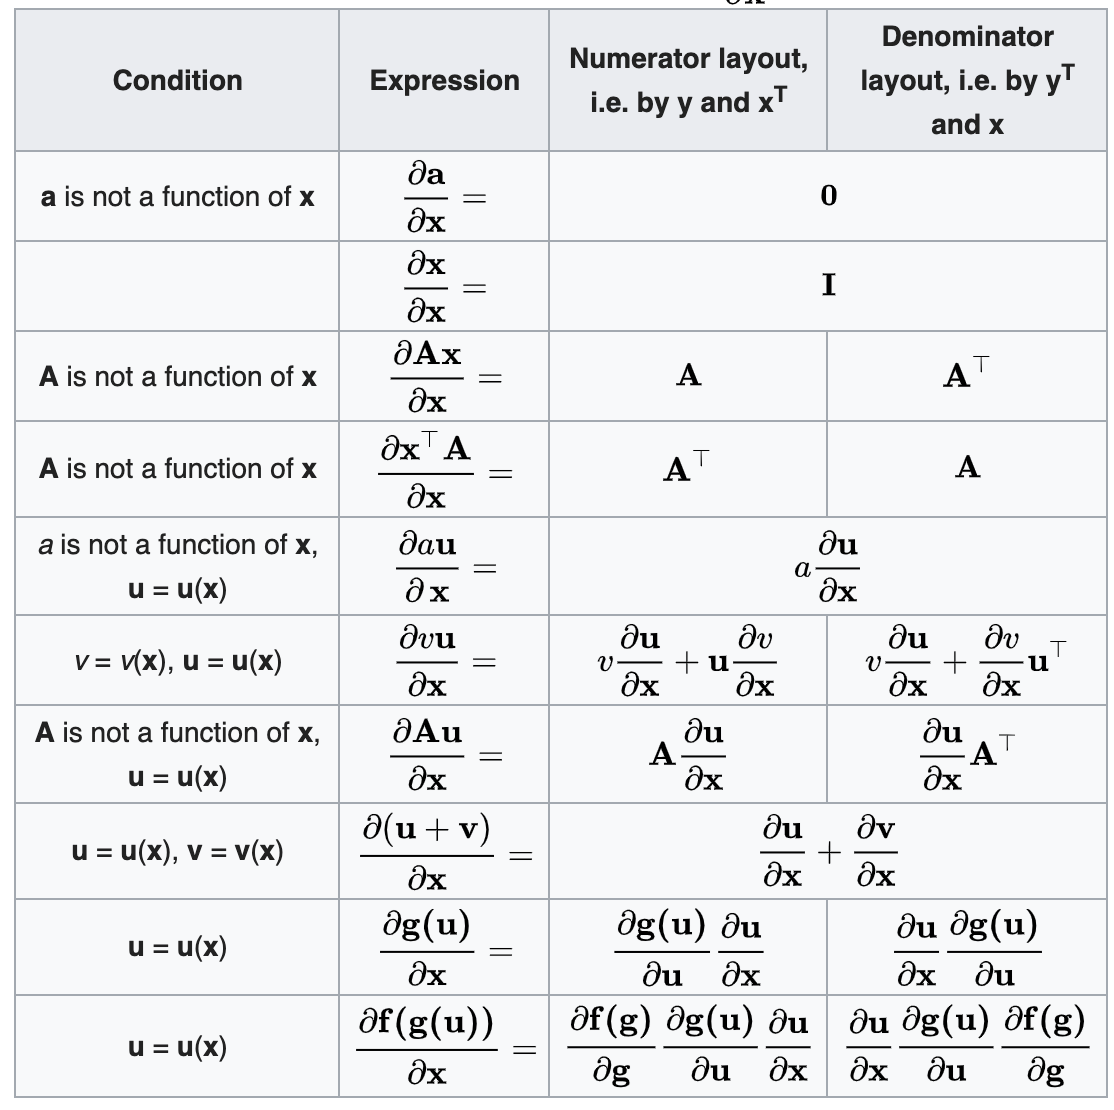
\includegraphics[scale=0.6]{p1.png}
\end{figure}

\paragraph{Young's Theorem 1.3.10}
i.e. Symmetry of second derivatives
$$[\nabla_{xy}f(x,y)]^T = \nabla_{yx}f(x,y)$$
\proof \\
This is straightforward by writing out the elements of the matrix. \qed


\section{Second-year Calculus Review}
functions $\real \rightarrow \real$
\subsection{Mean Value Theorem in 1 Dimension}
$g \in C^1$ on $\real$
$$\frac{g(x+h) - g(x)}{h} = g'(x + \theta h)$$
where $\theta \in (0,1)$ \\
Or equivalently,
$$g(x+h) = g(x) + hg'(x+\theta h)$$

\subsection{1st Order Taylor Approximation}
$g \in C^1$ on $\real$
$$g(x + h) = g(x) + hg'(x) + o(h)$$
where $o(h)$ is ``little $o$" of $h$, the error term.

\noindent Say a function $f(h) = o(h)$, this means $\underset{h \rightarrow 0}{\lim} \frac{f(h)}{h} = 0$\\
For example, for $f(h) = h^2$, we can say $f(h) = o(h)$, \\
since $\underset{h \rightarrow 0}{\lim} \frac{f(h)}{h} = \underset{h \rightarrow 0}{\lim} \frac{h^2}{h} = \underset{h \rightarrow 0}{\lim} h = 0$\\
\proof (Use MVT): \\
WTS : $g(x+h) - g(x) - hg'(x) = o(h)$
\begin{align*}
	\underset{h \rightarrow 0}{\lim} \frac{[g(x+h) - g(x)] - hg'(x)}{h} &= \underset{h \rightarrow 0}{\lim} \frac{[hg'(x+\theta h)] - hg'(x)}{h} \\
	&=\underset{h \rightarrow 0}{\lim} \, g'(x + \theta h) - g'(x) \\
	&=\underset{h \rightarrow 0}{\lim} \, g'(x) - g'(x) \\
	&= 0
\end{align*}
\qed

\subsection{2nd Order Mean Value Theorem}
$g \in C^2$ on $\real$
$$g(x + h) = g(x) + hg'(x) + \frac{h^2}{2} g'(x+\theta h)$$
for some $\theta \in (0,1)$ \\\\
\proof \\
WTS: $g(x+h) - g(x) - hg'(x) - \frac{h^2}{2}g''(x) = o(h^2)$
\begin{align*}
	\underset{h \rightarrow 0}{\lim} \frac{g(x+h) - g(x) - hg'(x) - \frac{h^2}{2}g''(x)}{h^2}
	&= \underset{h \rightarrow 0}{\lim} \frac{[\frac{h^2}{2}g'(x+\theta h)] - \frac{h^2}{2}g''(x)}{h^2}\\
	&=\underset{h \rightarrow 0}{\lim}\, \frac{1}{2}(g''(x+\theta h) - g''(x)) \\
	&=\underset{h \rightarrow 0}{\lim}\, \frac{1}{2}(g''(x) - g''(x)) \\
	&= 0
\end{align*}
\qed

multivariate functions: $\real^n \rightarrow \real$
\subsection{Recall: Definition of gradient}
Gradient of $f: \real^n \rightarrow \real$ at $x \in \real^n$ (denoted $\nabla f(x)$) if exists is a vector characterized by the property:
$$\underset{\vv \rightarrow \vo}{\lim} \frac{f(\vx+\vv)-f(\vx) - \nabla f(\vx) \cdot \vv}{||\vv||} = 0$$
In Cartesian coordinates, $\nabla f(\vx) = (\frac{\partial f}{\partial \vx_1}(\vx), \hdots, \frac{\partial f}{\partial \vx_n}(\vx))$

\subsection{Mean Value Theorem in $n$ dimension}
$f \in C^1$ on $\real^n$, then for any $\vx, \vv \in \real^n$,
$$f(\vx + \vv) = f(\vx) + \nabla f(\vx+ \theta \vv) \cdot \vv$$
for some $\theta \in (0,1)$\\\\
\proof Reduce to 1-dimension case \\
$g(t) := f(\vx+t\vv), t \in \real$ \\
\begin{align*}
	g'(t) &= \frac{d}{dt}f(\vx+t\vv) \\
	&= \sum_{i=1}^n \frac{\partial f}{\partial \vx_i}(\vx + t\vv)\cdot \frac{d(\vx+t\vv)_i}{dt}
	\tag{by Chain Rule} \\
	&= \sum \frac{\partial f}{\partial \vx_i}(\vx + t\vv)\cdot \frac{d(\vx_i + t\vv_i)}{dt} \\
	&= \sum \frac{\partial f}{\partial \vx_i} (\vx + t\vv)\cdot \vv_i \\
	&= \nabla f(\vx + t\vv)\cdot \vv \tag{*}
\end{align*}
$g \in C^1$ on $\real$\\
Using MVT in $\real$:
\begin{align*}
f(\vx+\vv) &= g(1) \\
&= g(0+1) \\
&= g(0) + 1g'(0+\theta 1) \tag{$\theta \in (0,1)$}\\
&= g(0) + g'(\theta) \\
&= f(\vx) + \nabla f(\vx+\theta \vv) \cdot \vv \tag{by (*)}
\end{align*}
\qed

\subsection{1st Order Taylor Approximation in $\real^n$}
$f \in C^1$ on $\real^n$
$$f(\vx + \vv) = f(\vx) + \nabla f(\vx) \cdot \vv + o(||\vv||)$$
\proof \\
\begin{align*}
	\underset{||\vv|| \rightarrow 0}{\lim} \frac{[f(\vx + \vv) - f(\vx)] - \nabla f(\vx) \cdot \vv }{||\vv||} 
	&= \underset{||\vv|| \rightarrow 0}{\lim} \frac{[\nabla f(\vx + \theta \vv) \cdot \vv] - \nabla f(\vx) \cdot \vv}{||\vv||} \\
	&= \underset{||\vv|| \rightarrow 0}{\lim} [\nabla f(\vx + \theta \vv) - \nabla f(\vx)] \cdot \frac{\vv}{||\vv||} \\
	&= 0 \tag{$\frac{\vv}{||\vv||}$ is a unit vector, remains 1}
\end{align*}
\qed
\subsection{2nd Order Mean Value Theorem in $\real^n$}
$f \in C^2$ on $\real ^n$
$$ f(\vx + \vv) = f(\vx) + \nabla f(\vx) \cdot \vv + \frac{1}{2}\vv^T\nabla^2 f(\vx + \theta \vv) \cdot \vv$$
\paragraph{Remarks}
In this course, \textcolor{red}{$\nabla^2$ means Hessian, not Laplacian.}
$$\nabla^2 f(\vx) =  \left( \frac{\partial^2 f}{\partial \vx_i \partial \vx_j}\right)_{1\leq i, j\leq n}(\vx) = \begin{pmatrix}
	\frac{\partial f}{\partial_1^2} & \frac{\partial f}{\partial_1 \partial_2} & \hdots \\
	\frac{\partial f}{\partial_2 \partial_1} & \hdots \\
	\vdots
\end{pmatrix}$$
The Hessian matrix is \textcolor{blue}{symmetric}. This is sometimes called \under{Clairaut's Theorem}.\\
\under{note}: $\vv^T \nabla^2 f(\vx)\vv = \sum_{1 \leq i, j\leq n} \frac{\partial^2 f}{\partial \vx_i \partial \vx_j}f(\vx)\vv_i \vv_j$

\subsection{2nd Order Taylor Approximation in $\real^n$}
$f \in C^2$ on $\real^n$ \\
$$f(\vx + \vv) = f(\vx) + \nabla f(\vx) \cdot \vv + \frac{1}{2}\vv^T\nabla^2 f(\vx) \vv + o(||\vv||^2)$$
\proof \\
\begin{align*}
	\underset{||\vv|| \rightarrow 0}{\lim} \frac{[f(\vx + \vv) - f(\vx)] - \nabla f(\vx)\cdot \vv - \frac{1}{2} \vv^T \nabla^2 f(\vx)\vv}{||\vv||^2} 
	&= \underset{||\vv|| \rightarrow 0}{\lim} \frac{[\frac{1}{2}\vv^T\nabla^2 f(\vx + \theta \vv) \cdot \vv] - \frac{1}{2}\vv^T\nabla^2 f(\vx) \cdot \vv}{||\vv||^2} \tag{By 2nd MVT}\\
	&=  \underset{||\vv|| \rightarrow 0}{\lim} \frac{1}{2}(\frac{\vv}{||\vv||})^T[\nabla^2 f(\vx + \theta \vv) - \nabla^2 f(\vx)](\frac{\vv}{||\vv||}) \\
	&= 0
\end{align*}
\qed 
\subsection{Geometric Meaning of Gradient}
$f: \real^n \rightarrow \real$\\
Rate of change of $f$ at $\vx$ in direction $\vv \, (||\vv||=1) = \frac{d}{dt}|_{t=0}f(\vx + t\vv)$
\begin{align*}
	\frac{d}{dt}|_{t=0}f(\vx + t\vv) &= \nabla f(\vx + t\vv) \cdot \vv |_{t=0} \\
	&= \nabla f(\vx)\cdot \vv \\
	&= |\nabla f(\vx)| |\vv| \cos \theta\\
	&= |\nabla f(\vx)| \cos \theta \tag{$||\vv||  = 1$}
\end{align*}
maximized at $\theta = 0$ \\
So $\nabla f(\vx)$ points in the direction of steepest ascent.

\subsection{Implicit Function Theorem}
$f: \real^{n+1} \rightarrow \real \in C^1$ \\
Fix $(\va,b) \in \real^n \times \real$ s.t. $f(\va,b) = 0$. \\
If $\nabla f(\va,b) \neq 0$, then $\{(\vx, y) \in (\real^n \times \real) | f(\vx, y) = 0\}$ is locally (near $(\va, b)$) the graph of a function.

\subsection{Level Sets of $f$}
$c$-level set of $f$ := $\{ \vx \in \real^n | f(\vx) = c\}$
\paragraph{Fact} gradient $\nabla f(\vx_0) \perp$ level curve (through $\vx_0$)

\section{Convex Sets \& Functions}
\subsection{Definitions}
\paragraph{Definition of Convex Set}
$\Omega \subseteq \real^n$ is a \under{convex set} if
$\vx_1, \vx_2 \in \Omega \Rightarrow s\vx_1 + (1-s)\vx_2 \in \Omega$ where $s \in [0,1]$
\paragraph{Definition of Convex Function}
A function $f: \text{convex } \Omega \subseteq \real^n$ is \under{convex} if 
$$f(s\vx_1 + (1-s)\vx_2) \leq sf(\vx_1) + (1-s)f(\vx_2)$$
for all $\vx_1, \vx_2 \in \Omega$ and all $s \in [0, 1]$
\paragraph{Remarks}
Second line above (or equal to) the graph
\paragraph{Definition of Concave Function}
A function $f$ is \under{concave} if $-f$ is convex.

\subsection{Basic Properties of Convex Functions}
Let $\Omega \subseteq \real^n$ be a convex set.
\begin{enumerate}
	\item $f_1, f_2$ are convex functions on $\Omega \Rightarrow f_1 + f_2$ is a convex function on $\Omega$.
	\item $f$ is a convex function, $a \geq 0 \Rightarrow af$ is a convex function.
	\item $f$ is a convex function on $\Omega \Rightarrow$ The sublevel sets of $f$, $SL_c:=\{\vx \in \real^n | f(\vx) \leq c\}$ is convex.
\end{enumerate}
\under{\ti{proof of (3):}} \\
Let $x_1, x_2 \in SL_C$, so that $f(x_1) \leq c$ and $f(x_2) \leq c$. \\
WTS: $sx_1 + (1-s)x_2 \in SL_c$ for any $s \in [0,1]$
\begin{align*}
	f(sx_1 + (1-s)x_2) &\leq sf(x_1) + (1-s)f(x_2) \tag{$f$ is convex}\\
	&\leq sc + (1-s)c \\
	&= c \\
\Rightarrow sx_1 + (1-s)x_2 \in SL_c
\end{align*}
\qed

\paragraph{Example of a convex function}
Let $f: \real \rightarrow \real, \,f(x) = |x|$ \\
Let $x_1, x_2 \in \real, s \in [0,1]$ \\
Then
\begin{align*}
	f(sx_1 + (1-s)x_2) &= |sx_1 + (1-s)x_2| \\
	&\leq |sx_1| + |(1-s)x_2| \tag{by Triangle Inequality}\\
	&= s|x_1| + (1-s)|x_2| \\
	&= sf(x_1) + (1-s)f(x_2)
\end{align*}
Then $f$ is a convex function.
\paragraph{Theorem - Characterization of $C^1$ convex functions}
Let $f: \text{convex subset of $\real^n$ } \Omega \rightarrow \real$ be a $C^1$ function. \\
Then,\\
$f$ is convex $\iff$ $f(y) \geq f(x) + \nabla f(x)\cdot(y-x)$ 
for all $x,y \in \Omega$
\paragraph{Remarks}
Tangent line below the graph.\\\\
\proof \\
($\Rightarrow$) \\
$f$ is convex, then by definition,
\begin{align*}
f(s\vx_1 + (1-s)\vx_2) &\leq sf(\vx_1) + (1-s)f(\vx_2)\\
f(s\vx_1 + (1-s)\vx_2) - f(\vx_2) &\leq s(f(\vx_1) - f(\vx_2)) \\
\frac{f(s\vx_1 + (1-s)\vx_2) - f(\vx_2)}{s} &\leq f(\vx_1) - f(\vx_2) \\
\underset{s \rightarrow 0}{\lim} \frac{f(\vx_2 + s(\vx_1 - \vx_2)) - f(\vx_2)}{s} &\leq f(\vx_1) - f(\vx_2) \\
\nabla f(\vx_2)\cdot(\vx_1 - \vx_2) &\leq f(\vx_1) - f(\vx_2) \tag{since $\frac{d}{ds}|_{s=0} f(\vx_2 + s(\vx_1 - \vx_2)) = \nabla f(\vx_2) \cdot (\vx_1 - \vx_2)$}\\
f(\vx_2) + \nabla f(\vx_2)\cdot(\vx_1 - \vx_2) &\leq f(\vx_1)\\
f(\vx) + \nabla f(\vx) \cdot (\vy-\vx) &\leq f(\vy)
\end{align*}
where $0\leq s \leq 1$ \\
($\Leftarrow$)\\
Fix $\vx_0, \vx_1 \in \Omega$ and $s \in (0,1)$ \\
Let $x = s\vx_0 + (1-s)\vx_1$ \\
$$\begin{cases}
	f(\vx_0) &\geq f(\vx) + \nabla f(\vx) \cdot (\vx_0 - \vx) \\
	&= f(\vx) + \nabla f(\vx) \cdot (1-s)(\vx_0 - \vx_1) \\
	f(\vx_1) &\geq f(\vx) + \nabla f(\vx) \cdot (\vx_1 - \vx) \\
	&= f(\vx) + \nabla f(\vx) \cdot s(\vx_1 - \vx_0) \\
\end{cases}$$
	$$\begin{cases}sf(x_0) &\geq sf(\vx) + \nabla f(\vx) \cdot (1-s) \cdot s(\vx_0 - \vx_1) \\
	(1-s)f(\vx_1) &\geq (1-s)f(\vx) + \nabla f(\vx) \cdot (1-s)\cdot s(\vx_1 - \vx_0)  \end{cases}$$
Then
$$sf(\vx_0) + (1-s)f(\vx_1) \geq f(x) + 0$$
Then $f$ is convex.
\qed

\subsection{Criterions for convexity}
\paragraph{$C^1$ criterion for convexity}
$$f: \Omega \rightarrow \real \text{ is convex } \iff f(y) \geq f(x) + \nabla f(x) \cdot (y-x)$$
for all $x, y \in \Omega$

\paragraph{Theorem: $C^2$ criterion for convexity}
Let $f \in C^2$ on $\Omega \subseteq \real^n$ (here we assume $\Omega \subseteq \real^n$ is a convex set containing an interior point) \\
Then $$f \text{ is convex on } \Omega \iff \nabla^2 f(x) \geq 0$$ for all $x \in \Omega$


\paragraph{Remark 1}
Let $A$ be an $n \times n$ matrix.\\
``$A \geq 0$" means $A$ is positive semi-definite:
$$v^TAv \geq 0$$ for all $v \in \real^n$

\paragraph{Remark 2}
In $\real$, 
$$f \text{ is convex } \iff f'(x) \geq 0$$ for all $x \in \Omega$ \\
(``concave up" in first year calculus) \\\\
\ti{\under{proof for Theorem:}} \\
Recall 2nd order MVT: \\
$$f(y) = f(x) + \nabla f(x)\cdot (y-x) + \frac{1}{2}(y-x)^T \nabla^2 f(x+s(y-x))\cdot (y-x)$$
for some $s \in [0,1]$ \\
($\Leftarrow$) \\
Since $\nabla^2 f(x) \geq 0$, then 
$$\frac{1}{2}(y-x)^T \nabla^2 f(x+s(y-x))\cdot (y-x) \geq 0$$
Then
$$f(y) \geq f(x) + \nabla f(x) \cdot (y-x)$$
for all $x, y \in \Omega$. \\
Then by $C^1$ criterion,
$f$ is convex. \\
($\Rightarrow$) \\
Assume $f$ is convex on $\Omega$. \\
Suppose for contradiction that $\nabla^2 f(x)$ is not positive semi-definite at some $x \in \Omega$. \\
Then $\exists v \neq 0$ s.t. $v^T \nabla^2f(x) v < 0$
$v$ could be arbitrarily small and $>0$\\
Let $y = x + v$, then
$$(y-x)^T\nabla^2 f(x + s(y-x))\cdot (y-x) < 0$$
for all $s \in [0,1]$ \\
Then by MVT,
$$f(y) < f(x) + \nabla f(x)\cdot(y-x)$$
for some $x, y \in \Omega$, and this contradicts the $C^1$ criterion. \qed

\subsection{Minimization and Maximization of Convex Functions}
\paragraph{Theorem}
$f:$ convex $\Omega \subseteq \real^n \rightarrow \real$ is a convex function. \\
Suppose $\Gamma := \{ x \in \Omega | f(x) = \underset{\Omega}{\min} \, f(x)\} \neq \emptyset$\\
(i.e. minimizer exists) \\
Then $\Gamma$ is a convex set, and any local minimum of $f$ is a global minimum of $f$. \\
\proof \\\\
Let $m = \underset{\Omega}{\min} f(x)$.
$$\Gamma = \{ x \in \Omega | f(x) = m\} = \{ x \in \Omega | f(x) \leq m \}$$
(sublevel set) \\
Then by Basic Properties of Convex Sets, $\Gamma$ is convex. \\
Let $x$ be a local minimum of $f$.\\
Suppose for contradiction that $\exists y$ s.t. $f(y) < f(x)$ \\
(i.e. $x$ is not a global minimum)
\begin{align*}
	f(sy + (1-s)x) &\leq sf(y) + (1-s)f(x) \\
	&< sf(x) + (1-s)f(x) \tag{$f(y) < f(x)$}\\
	&= f(x)
\end{align*}
for all $s \in (0,1)$ \\
As $s$ approaches 0, $s$ approaches $x$. \\
Then we have
$\underset{s \rightarrow 0}{\lim} f(sy + (1-s)x) = f(x) < f(x)$.\\
which is a contradiction. \qed


\paragraph{Theorem}
If $f: \Omega \subseteq \real^n \rightarrow \real$ is a convex function, and $\Omega$ is convex and compact, then $$\underset{\Omega}{\max} f = \underset{\partial \Omega}{\max} f$$
\paragraph{Remarks}
Maximum value of $f$ is attained (also) on the boundary of $\Omega$ \\
\proof \\
Since $\Omega$ is closed, $\partial \Omega \subseteq \Omega$, so $\underset{\Omega}{\max} f \geq \underset{\partial \Omega}{\max} f$.\\
Suppose $f(x_0) = \underset{\Omega}{\max} \, f$ for some $x_0 \notin \partial \Omega$.
Let $L$ be an arbitrary line through $x_0$. \\
By convexity and compactness of $\Omega$, L meets $\partial \Omega$ at two points $x_1, x_2$. 
\\
Let $x_0 + sx_1 + (1-s)x_2$ for $ s\in (0,1)$
\begin{align*}
	f(x_0) &= f(sx_1 + (1-s)x_2) \\
	&\leq sf(x_1) + (1-s)f(x_2) \tag{$f$ convex}\\
	&\leq \max\{f(x_1), f(x_2)\} \\
	&\leq \underset{\partial \Omega}{\max} \, f\\
	&\leq \underset{\Omega}{\max} \, f = f(x_0) 
\end{align*}
This implies that $$\underset{\Omega}{\max} \, f = \underset{\partial \Omega}{\max} \, f$$
as wanted.
\qed

\paragraph{Example}
$$|ab| \leq \frac{1}{p}|a|^p + \frac{1}{q}|b|^q$$
where $p,q > 1$ s.t. $\frac{1}{p} + \frac{1}{q} = 1$.\\
\under{Special cases:}
\begin{enumerate}
	\item $$p=q=2, |ab| \leq \frac{|a|^2 + |b|^2}{2}$$ 
	\item 
	$$p=3, q=\frac{3}{2}, |ab| \leq \frac{1}{3}|a|^3 + \frac{2}{3}|b|^{\frac{3}{2}}$$
\end{enumerate}
\proof \\
Since function $f(x) = -\log (x)$ is convex, then
\begin{align*}
	(-\log)|ab| &= (-\log)|a| + (-\log)|b| \\
	&= \frac{1}{p}(-\log)|a|^p + \frac{1}{q}(-\log)|b|^q \\
	&\geq (-\log)(\frac{1}{p}|a|^p + \frac{1}{q}|b|^q)\\
	(-\log)|ab| &\geq (-\log)(\frac{1}{p}|a|^p + \frac{1}{q}|b|^q) \\
	\log|ab| &\leq \log(\frac{1}{p}|a|^p + \frac{1}{q}|b|^q) \\
	|ab| &\leq \frac{1}{p}|a|^p + \frac{1}{q}|b|^q \tag{exponential function is increasing}
\end{align*}
\qed 
\section{Basics of Unconstrained Optimization}
\subsection{Extreme Value Theorem}
Suppose $f: \real^n \rightarrow \real$ is continuous, and compact set $K \subseteq \real^n$
Then the problem
$$\underset{x \in K}{\min} \, f(x)$$ has a solution.

\paragraph{Recall}
\begin{enumerate}
	\item $$K \subseteq \real^n \text{ compact} \iff K \text{ closed and bounded}$$
	\item If $h_1, \hdots, h_k$ and $g_1, \hdots, g_m$ are continuous functions on $\real^n$, then the set of all points $x \in \real^n$ s.t.
	$$\begin{cases}
		h_i(x) = 0  &\text{for all $i$} \\
		g_j(x) \leq 0 &\text{for all $j$}
	\end{cases}$$
	is a closed set.
	\item If such a set is also bounded, then it is compact.
\end{enumerate}

\paragraph{Example}
$$\{(x,y) \in \real^2 | x^2 + y^2 -1 = 0 \}$$
by (2), this is a closed set \\
by (3), this is a compact set.

\paragraph{Remarks}
$f: \Omega \subseteq \real^n \rightarrow \real$ convex does not imply $f$ is continuous.

\subsection{Unconstrained Optimization}
$$\underset{x \in \Omega \subseteq \real^n}{\min f(x)}$$
typically
\begin{enumerate}
	\item $\Omega \subseteq \real^n$
	\item $\Omega = \real^n$
	\item $\Omega = $ open
	\item $\Omega = \overline{\text{open}}$ 
\end{enumerate}

\paragraph{Remark}
\begin{enumerate}
	\item $\max f(x) = - (\min - f(x))$
	\item $\min f(x) = - (\max - f(x))$
\end{enumerate}

\paragraph{Definition: local minimum}
We say that $f$ has a \under{local minimum} at a point $x_0 \in \Omega$ if
$$f(x_0) \leq f(x)$$ for all $x \in B_{\Omega}^\varepsilon (x_0)$, where $B_{\Omega}^\varepsilon (x_0) = \{ x \in \Omega: |x - x_0| < \varepsilon\}$ which is an open ball around $x_0$ inside $\Omega$ of radius $\varepsilon >0$. \\
We say that $f$ has a \under{strict local minimum} at a point $x_0 \in \Omega$ if
$$f(x_0) < f(x)$$ for all $x \in B_{\Omega}^\varepsilon (x_0) \setminus \{x_0\}$

\subsection{1st order necessary condition for local minimum}
\paragraph{Theorem} Let $f$ be a $C^1$ function on $\Omega \subseteq \real^n$. If $x_0 \in \Omega$ is a local minimum of $f$, then
$$ \nabla f(x_0) \cdot v \geq 0$$
for all feasible directions $v$ at $x_0$

\paragraph{Definition: feasible direction}
$v \in \real^n$ is a \under{feasible direction} at $x_0 \in \Omega$ if $$x_0 + sv \in \Omega$$ for all $0 \leq s \leq \bar{s}$ where $\bar{s} \in \real$
\paragraph{Remarks}
\textcolor{red}{Feasible directions go into the set.}
\paragraph{Corollary}
Special case: If $\Omega = \real^n$ is an open set, then any direction is a feasible direction.
Then $x_0$ is a local minimum of $f$ on $\Omega$ implies that $\nabla f(x_0) \cdot v \geq 0$ for all $v \in \real^n$.
$$\begin{cases}
	\nabla f(x_0) \cdot v \geq 0 \\
	\nabla f(x_0) \cdot (-v) \geq 0 \iff \nabla f(x_0) \cdot v \leq 0
\end{cases} \implies \nabla f(x_0) \cdot v = 0 \text{ for all $v \in \real^n$}$$
$$\implies \nabla f(x_0) = 0$$
\begin{proof}
[ ]
\end{proof}

\subsection{2nd order necessary condition for local minimum}
$f \in C^2, \Omega \subseteq \real^n$ \\
If $x_0 \in \Omega$ is a local minimum of $f$ on $\Omega$, then
\begin{enumerate}
	\item $\nabla f(x_0) \cdot v \geq 0$ for al feasible directions $v$ at $x_0$
	\item If $\nabla f(x_0) \cdot v = 0$, then $v^T \nabla^2 f(x_0) v \geq 0$
	(function curves up)
\end{enumerate}
\begin{proof}
[]
\end{proof}

\paragraph{Remark}
If $x_0$ is an interior point of $\Omega$, then
$$\nabla f(x_0) = 0, \quad \nabla^2 f(x_0)\geq 0$$
$$f'(x_0) = 0, \quad f''(x_0) \geq 0$$

\paragraph{Definition: principal minor}
Let $A$ be an $n \times n$ matrix. A $k \times k$ submatrix of $A$ formed by deleting $n-k$ rows of $A$, and the \textcolor{red}{same} $n - k$ columns of $A$, is called \under{principal submatrix} of $A$. The determinant of a principal submatrix of $A$ is called a \under{principal minor} of $A$.

\paragraph{Definition: leading principal minor}
Let $A$ be an $n \times n$ matrix. The $k$th order principal submatrix of $A$ obtained by deleting the \textcolor{red}{last} $n-k$ rows and columns of $A$ is called the $k$-th order \under{leading principal submatrix} of $A$, and its determinant is called a \under{leading principal minor} of $A$.

\paragraph{Definition: positive definiteness (Sylvester's Criterion)}
A $n \times n$ matrix $A$ is \\
\begin{enumerate}
	\item \under{positive definite} if $v^TAv > 0$ for all $v \neq 0 \iff $ all eigenvalues $>0$ $\iff$ \textcolor{red}{all leading principle minors $> 0$}
	\item \under{positive semi-definite} if $v^TAv \geq 0$ for all $v \iff $ all eigenvalues $\geq 0$ $\iff$ \textcolor{red}{all principle minors $\geq 0$}
\end{enumerate}

\paragraph{Lemma}
Suppose $\nabla^2 f(x_0)$ is positive definite, then
$$\exists a > 0 \,\, s.t. \,\, v^T\nabla^2f(x_0)v \geq a||v||^2 \quad \forall v$$


\subsection{2nd order sufficient condition (for interior points)}
$f \in C^2$ on $\Omega$ \\
If $\begin{cases}
	\nabla f(x_0) = 0 \\
	\nabla^2 f(x_0) > 0
\end{cases},$ then $x_0$ is a strict local minimum. \\
\begin{proof}
	[ ]
\end{proof}


\section{Optimization with Equality Constraints}

\subsection{Definitions of Related Spaces}
\paragraph{Definition 5.1.1: surface}
$$M =  \text{``surface"}  = \{ x \in \real^n | h_1(x) = 0, \hdots, h_k(x) = 0\}$$ 
where $h_i \in C^1$

\paragraph{Definition 5.1.2: differentiable curve on surface}
A \under{differentiable curve} on surface $M \subseteq \real^n$ is a $C^1$ function
$$ x: (-\epsilon, \epsilon) \rightarrow M: s \mapsto x(s)$$ 
\paragraph{Remarks}
\begin{enumerate}
	\item Let $x(s)$ be a differentiable curve on $M$ that passes through $x_0 \in M$, say $x(0) = x_0$. The vector $v = \frac{d}{ds}|_{s=0} \, x(0)$ touches M ``tangentially". We say $v$ is generated by $x(s)$.
	\item In previous calculus courses, differentiable curves are often referred to as parameterizations.
\end{enumerate}
\paragraph{Definition 5.1.3: tangent vector}
Any vector $v$ which is generated by some differentiable curve on $M$ through $x_0$ is called a \under{tangent vector}.

\paragraph{Definition 5.1.4: tangent space}
\under{Tangent space} to the surface $M$ at point $x_0$ is
$$T_{x_0} M = \{ \text{all tangent vectors to $M$ at $x_0$} \} \\
= \{v \in \real^n: v = \frac{d}{ds} |_{s=0} \, x(s)\}$$
where $x(s)$ is a differentiable curve on $M$ s.t. $x(0) = x_0$

\paragraph{Remarks}
The zero vector is contained in all tangent spaces.

\paragraph{Definition 5.1.5: T-space}
$$T_{x_0} = \{ x\in \real^n: x^T \nabla h_i(x_0) = 0 \, \forall i\} = Span\{ \nabla h_1(x_0), \hdots, \nabla h_k(x_0)\}^\perp$$

\paragraph{Definition 5.1.6: regular point}
$x_0 \in M$ is a \under{regular point} (of the constraints) if $\{ \nabla h_1(x_0), \hdots. \nabla h_k(x_0) \}$ are linearly independent.
\paragraph{Remark}
If there is only one constraint $h$, then $x_0$ is regular if and only if $\nabla h(x_0) \neq 0$.

\paragraph{When does the T-space equivalent to the tangent space?}
\textcolor{red}{When $x_0$ is a regular point (of the constraints).}

\paragraph{Theorem 5.1.7}
Suppose $x_0$ is a regular point s.t. $ M = \{ x \in \real^n: h_i(x) = 0 \, \forall i\}$. Then
$$T_{x_0}M = T_{x_0}$$

\paragraph{Lemma 5.1.8}
$f, h_1, \hdots, h_k \in C^1$ on open $\Omega \subseteq \real^n$ \\
$ M = \{ x \in \real^n: h_i(x) = 0 \, \forall i\}$ \\
Suppose $x_0 \in M$ is a local minimum of $f$ on $M$, then
$$\nabla f(x_0) \perp T_{x_0}M \iff \nabla f(x_0)\cdot v = 0$$ for all $v \in T_{x_0}M$

\subsection{Lagrange Multipliers: 1st order necessary condition for local minimum}
$f, h_1, \hdots, h_k \in C^1$ on open $\Omega \subseteq \real^n$. \\
Let $x_0$ be a regular point of the constraints $ M = \{ x \in \real^n: h_i(x) = 0 \, \forall i\}$. \\
Suppose $x_0$ is a local minimum of $f$ on $M$, then $\exists \lambda_1, \hdots, \lambda_k \in \real$ s.t.
$$\nabla f(x_0) + \lambda_1 \nabla h_1(x_0) + \hdots + \lambda_k \nabla h_k(x_0) = 0$$
\begin{proof}
	$x_0$ regular implies that $$\tanspace = \tspace = Span\{\nabla h_1(x_0), \hdots, \nabla h_k(x_0)\}^\perp$$
	By Lemma 5.1.8, $x_0$ is a loc min implies that $$\nabla f(x_0) \perp \tanspace$$
	Then $$\nabla f(x_0) \in (\tanspace)^\perp = Span\{\nabla h_i (x_0)\}^{\perp\perp} = Span\{ \nabla h_i(x_0)\}$$
	Then 
	$$\nabla f(x_0) = -\lambda_1 \nabla h_1(x_0) - \hdots - \lambda_k \nabla h_k(x_0)$$
	for some $\lambda_i \in \real$ \qed
\end{proof} 

\subsection{2nd order necessary condition for local minimum}
$f, h_1, \hdots, h_k \in \textcolor{red}{C^2}$ on open $\Omega \subseteq \real^n$. \\
Let $x_0$ be a regular point of the constraints $ M = \{ x \in \real^n: h_i(x) = 0 \, \forall i\}$. \\
Suppose $x_0$ is a local minimum of $f$ on $M$, then
\begin{enumerate}
	\item $$\nabla f(x_0) + \sum_{i=1}^k \lambda_i \nabla h_i(x_0) = 0$$
	for some $\lambda_i \in \real$
	\item \textcolor{blue}{$$\nabla^2 f(x_0) + \sum \lambda_i \nabla^2 h_i(x_0) \geq 0$$ on $T_{x_0}M$}
\end{enumerate}

\subsection{2nd order sufficient condition for local minimum}
$f, h_1, \hdots, h_k \in \textcolor{red}{C^2}$ on open $\Omega \subseteq \real^n$. \\
Let $x_0$ be a regular point of the constraints $ M = \{ x \in \real^n: h_i(x) = 0 \, \forall i\}$. \\
If $\exists \lambda_i \in \real$ s.t.
\begin{enumerate}
	\item $$ \nabla f(x_0) + \sum \lambda_i \nabla h_i(x_0) = 0$$
	\item $$ \nabla^2 f(x_0) + \sum \lambda_i \nabla^2 h_i(x_0) \textcolor{red}{>} 0$$ on $T_{x_0} M$
\end{enumerate}
Then $x_0$ is a strict local minimum.\\\\
\begin{proof}
	Recall that (2) means $[\nabla^2 f(x_0) + \sum \lambda_i h_i(x_0)]$ is pos-def on $T_{x_0}M$. \\
	Then $ \exists a > 0$ s.t. $v^T [\nabla^2 f(x_0) + \sum \lambda_i h_i(x_0)] v \geq a||v||^2$ for all $v \in \tanspace$. \\
	Let $x(s) \in M$ be a curve s.t. $x(0) = x_0$ and $v = x'(0)$. \\
	WLOG, $||x'(0)|| = 1$.\\
	By 2nd order Taylor, 
	\begin{align*}
		f(x(s)) - f(x(0)) &= s\frac{d}{ds}|_{s=0} f(x(s)) + \frac{1}{2} s^2 \frac{d}{ds^2} |_{s=0} f(x(s)) + o(s^2)\\
		&= s\frac{d}{ds}|_{s=0} [f(x(s)) + \sum_i \lambda_i h_i(x(s)) ]+ \frac{1}{2} s^2 \frac{d}{ds^2}|_{s=0} [f(x(s)) + \sum_i \lambda_i h_i(x(s)) ] + o(s^2) \tag{$\sum_i \lambda_i h_i(x(s)) = 0$}\\
		&=  s[\nabla f(x_0) + \sum \lambda_i \nabla h_i(x_0)] \cdot x'(0) + \frac{1}{2}s^2x'(0)^T[\nabla^2f(x_0) + \sum \lambda_i \nabla^2h_i(x_0)] x'(0) + o(s^2) \\
		&= 0 + \frac{1}{2} s^2 v^T[\nabla^2f(x_0) + \sum \lambda_i \nabla^2h_i(x_0)]v + o(s^2) \\
		&\geq \frac{1}{2}s^2 a||v||^2 + o(s^2) \\
		&= \frac{1}{2}s^2 a + o(s^2) \\
		&= s^2 [\frac{a}{2} + \frac{o(s^2)}{s^2}] > 0
	\end{align*}
	for small $s >0$, since $\frac{a}{2} > 0$ and $\underset{s \rightarrow 0}{\lim} \frac{o(s^2)}{s^2} = 0$ \\
	Then $f(x(s)) > f(x_0)$ for small $s > 0$
	Then $x_0$ is a strict local min of $f$. \qed
\end{proof}


\section{Optimization with Inequality Constraints}
\paragraph{Problem}
open $\Omega \subseteq \real^n$\\
$f: \Omega \rightarrow \real$ \\
$h_1, \hdots, h_k: \Omega \rightarrow \real$ \\
$g_1, \hdots, g_l: \Omega \rightarrow \real$ \\
$$\begin{cases}
	\min f(x) \\
	x \in \Omega \text{ subject to } 
\begin{cases}
	h_1(x) = 0, \hdots, h_k(x) = 0 \\
	g_1(x) \leq 0, \hdots, g_l(x) \leq 0
\end{cases}
\end{cases}(*)$$

\paragraph{Definition 1: activeness}
Let $x_0$ satisfy the constraints. \\
We say that the constraint $g_i(x) \leq 0$ is \under{active} at $x_0$ if $g_i(x_0) = 0$. \\ It is \under{inactive} at $x_0$ if $g_i(x_0) < 0$.\\
\paragraph{Definition 2: regular point}
Suppose for some $l' \leq l$:
$$g_1(x) \leq 0, \hdots, g_{l'}(x) \leq 0; \, g_{l' + 1}(x) \leq 0, \hdots, g_l(x) \leq 0$$
where $g_1, \hdots g_{l'}$ active and the rest inactive. \\
We say that $x_0$ is a \under{regular point} of the constraints if \\
$\{\nabla h_1(x_0), \hdots, \nabla h_k(x_0), \nabla g_1(x_0), \hdots, \nabla g_{l'}(x_0)\}$ is linearly independent.

\subsection{Kuhn-Tucker conditions: 1st order necessary condition for local minimum}
open $\Omega \subseteq \real^n$\\
$f: \Omega \rightarrow \real$ \\
$h_1, \hdots, h_k, g_1, \hdots, g_l: C^1 \in \Omega$ \\
Suppose $x_0 \in \Omega$ is a regular point of the constraints which is a local minimum, then
\begin{enumerate}
	\item $$\nabla f(x_0) + \sum_{i=1}^k \lambda_i \nabla h_i(x_0) + \sum_{j=1}^l \mu_j \nabla g_j(x_0) = 0$$ for some $\lambda_i \in \real$ and \textcolor{red}{$\mu_j \geq 0$}
	\item $\mu_j g_j(x_0) = 0$
\end{enumerate}

\paragraph{Remark 1}
Given $x_0$, 
$$
\begin{cases}
g_j(x) \leq 0 \text{ active at } x_0 \implies g_j(x_0) = 0 \implies \mu_jg_j(x_0) = 0 \\
g_j(x) \leq 0 \text{ inactive at } x_0 \implies g_j(x_0) < 0 \implies \mu_j = 0
\end{cases}
$$
$\implies \mu_j = 0$ for all inactive $g_j$ at $x_0$

\paragraph{Remark 2}
It is possible for an active constraint to have zero multiplier.

\paragraph{Remark 3}
$\mu_j \geq 0$ because $\nabla f$ and $\nabla g$ have opposite directions at a local minimum $x_0$. \\
$$\nabla f(x_0) + \mu \nabla g(x_0) = 0 \implies \nabla f(x_0) = -\mu \nabla g(x_0) \implies -\mu < 0 \implies \mu > 0 $$
\textcolor{red}{Is this true?}

\paragraph{Idea of proof}
$x_0$ is a local min of $f$ subject to (*) \\
$\implies x_0$ is a local min for equality constraints $h_1(x) = 0, \hdots, h_k(x) = 0 +$ active inequality constraints $g_1(x) \leq 0, \hdots, g_{l'}(x) \leq 0$ \\
$\implies x_0$ is a local min for $h_1(x) = 0, \hdots, h_k(x) = 0 + g_1(x) = 0, \hdots, g_{l'}(x) = 0$ 
$\implies \nabla f(x_0) + \sum_{i=1}^k \lambda_i \nabla h_i(x_0) + \sum_{j=1}^{l'} \mu_j \nabla g_j(x_0) = 0$\\
for some $\lambda_i \in \real$ and $\mu_j \in \real$.\\
Let $\mu_j = 0$ for $j = l' + 1, \hdots, l$,
then 
$$\nabla f(x_0) + \sum_{i=1}^k \lambda_i \nabla h_i(x_0) + \sum_{j=1}^{\textcolor{red}{l}} \mu_j \nabla g_j(x_0) = 0$$

\subsection{2nd order necessary conditions for local minimum}
Open $\Omega \subseteq \real^n, f, h_1, \hdots, h_k, g_1, \hdots, g_l \in C^2$.
Let $x_0$ be a regular point of the constraints:
$$(+)\begin{cases}
	h_1(x) = \hdots = h_k(x_0) = 0 \\
	g_1(x), \hdots g_l(x_0) \leq 0
\end{cases}$$
Suppose $x_0$ is a local min of $f$ subject to (+).
Then, $\exists \lambda_i \in \real, \mu_j \geq 0$ s.t.
\begin{enumerate}
	\item $\nabla f(x_0) + \sum_{i=1}^k \lambda_i \nabla h_i(x_0) + \sum_{j=1}^l \mu_j \nabla g_j(x_0) = 0$
	\item $\mu_j g_j(x_0) = 0 $ for all $j$
	\item \textcolor{red}{$[\nabla^2 f(x_0) + \sum \lambda_i \nabla^2h_i(x_0) + \sum \mu_j \nabla^2 g_h(x_0)]]$ is positive semi definite on tangent space to active constraints at $x_0$.}
\end{enumerate}
\begin{proof}
	$x_0$ local min for ($\dag$) \\
	$\implies x_0$ local min for only active constraints at $x_0$. \\
	$\implies \begin{cases}
		h_i(x) = 0 \,\, \forall i \\
		g_j(x) = 0 \,\, j=1, \hdots, l'
	\end{cases}$ \\
	$\implies [\nabla^2 f(x_0) + \sum \lambda_i \nabla^2h_i(x_0) + \sum \mu_j \nabla^2 g_h(x_0)]]$ pos semi def on tangent space to active constraints. \qed
\end{proof}

\subsection{2nd order sufficient conditions}
Open $\Omega \subseteq \real^n, f, h_i, g_j \in C^2$ on $\Omega$. \\
\under{Problem:}
$$\begin{cases}
	\min &f(x) \\
	\text{subject to }&\begin{cases}h_i(x) = 0 \\
	g_j(x) \leq 0 \end{cases}
\end{cases}$$
Suppose $\exists x_0$ feasible and $\lambda_i, \mu_j \in \real$ s.t. 
\begin{enumerate}
	\item $\nabla f(x_0) + \sum_{i=1}^k \lambda_i \nabla h_i(x) + \sum_{j=1}^l \mu_j \nabla g_j(x_0) = 0$
	\item $\mu_j g_j(x_0) =0$ all $j$
\end{enumerate}
If the Hessian matrix, $L(x_0) = \nabla^2 f(x_0) + \sum_{i=1}^k \lambda_i \nabla^2 f(x_0) + \sum_{i=1}^l \mu_j \nabla^2 g_j(x)$ is pos def on $\tilde{\tilde{T}}_{x_0}$-space of ``strongly active" constraints at $x_0$. \\
Then $x_0$ is a strict local min. \\

\paragraph{Remarks}
\begin{enumerate}
	\item $$\text{Active constraints at $x_0$} \begin{cases}
	h_i(x) = 0 \quad i=1,\hdots,k \\
	g_j(x) \leq 0 \quad j = 1,\hdots, l' \implies g_j(x_0) = 0
	\end{cases}$$

	\item $$\text{\textcolor{red}{Strongly active constraints at $x_0$}} 
	\begin{cases}
	h_i(x) = 0 \quad i=1,\hdots,k \\
	g_j(x) \leq 0 \quad j = 1,\hdots, l'' \,\,\, \text{$g_j(x)$ is active at $x_0 \& \mu_j > 0$}
	\end{cases}$$
	$l'' \leq l' \leq l$
	\item $$\tilde{\tilde{T}}_{x_0} = \{ v\in \real^n | v\cdot \nabla h_i(x_0) = 0 \text{ all $i$} \& v \cdot \nabla g_j(x_0) = 0 \text{all $j = 1, \hdots, l''$} \}$$
	\item strongly active $\subseteq$ active \\
	      (strongly active)$^\perp \supseteq$ (active)$^\perp$
\end{enumerate}
\begin{proof}
	(details see another pdf by prof)
	Suppose $x_0$ is \textcolor{red}{NOT} a (strict) local min.
	\under{claim:} $\exists$ unit vector $v \in \real$ s.t.
	\begin{enumerate}
		\item $\nabla f(x_0) \cdot v \leq 0$
		\item $\nabla h_i(x_0) \cdot v = 0 \quad i = 1, \hdots, k$
		\item $\nabla g_j(x_0) \cdot v \leq 0 \quad j = 1, \hdots, l'$
	\end{enumerate}
	\under{proof of claim}: [] \\
	\under{claim:} $\nabla g_j(x)\cdot v = 0$ for $j = 1, \hdots, l''$ \\
	\under{proof of claim:} [] \\
	$\implies$ contradiction! \\
	\under{claim:} $\exists$ unit vector $v \in \real$ s.t.
	\begin{enumerate}
		\item $\nabla f(x_0) \cdot v \leq 0$
		\item $\nabla h_i(x_0) \cdot v = 0 \quad i = 1, \hdots, k$
		\item $\nabla g_j(x_0) \cdot v = 0 \quad j = 1, \hdots, l''$
	\end{enumerate}
	\under{proof of claim:} [] 
	\qed
\end{proof}


\section{Different Computation Methods for Solving Optimum}
\subsection{Newton's Method}
$x_0 \in I$ start \\
$x_{n+1} = x_0 - \frac{f'(x_0)}{f''(x_0)}$

\paragraph{Theorem}
Let $f \in C^3$ on $I$.\\
Suppose $x_* \in I$ satisfies $f'(x_*) = 0$ and $f''(x_*) \neq 0$ (\textcolor{red}{$x_*$ is a non-degenerate critical point}).\\
Then the sequence of points $\{x_n\}$ generated by Newton's method 
$$x_{n+1} = x_n  - \frac{f'(x_0)}{f''(x_0)}$$ converges to $x_*$ if $x_0$ is sufficiently close to $x_*$.

\paragraph{Why do we need this method?}
In real life, we may not know the real function formula. We only have data, using which we can approximate the function formula. In a way, Newton's method is true ``applied mathematics".

\paragraph{Proof of Theorem}
Let $g(x) = f'(x)$ so that $x_{n+1} = x_n - \frac{g(x_n)}{g'(x_n)}$ \\
By $g \in C^2, \exists \alpha$ s.t. $|g'(x_1)| > \alpha \, \forall x_1$ and $|g''(x_2)| < \frac{1}{\alpha} \,\, \forall x_2$ in a neighbourhood of $x_*$ (choose $\alpha$ small enough).

\begin{align}
	x_{n+1} - x_* &= x_n - \frac{g(x_n)}{g'(x_n)} - x_* \\
	&= x_n - x_* - \frac{g(x_n) - g(x_*)}{g'(x_n)} &\text{($g(x_*) = 0$)}\\
	&= \frac{-[g(x_n) - g(x_*) - g'(x_n)(x_n - x_*)]}{g'(x_n)} \\
	&= \frac{1}{2}\frac{g''(\xi)}{g'(x_n)}(x_n - x_*)^2 \\
	|x_{n+1} - x_*| &= \frac{1}{2}\frac{g''(\xi)}{g'(x_n)}|x_n - x_*|^2 < \frac{1}{2\alpha^2}|x_n - x_*|^2 &\text{(in small neighbourhood of $x_*$)} \\
	\rho &:= \frac{1}{2\alpha^2} |x_0 - x_*| &\text{(choose $x_0$ sufficiently close to $x_*$ s.t. $\rho < 1$)} \\
	|x_1 - x_*| &< \frac{1}{2\alpha^2}|x_0 - x_*|^2 \\
	&= \frac{1}{2\alpha^2}|x_0 - x_*||x_0 - x_*| \\
	&= \rho|x_0 - x_*| \\
	|x_2 - x_*| &< \frac{1}{2\alpha^2}|x_1 - x_*|^2 \\
	&< \frac{1}{2\alpha^2}\rho^2|x_0 - x_*|^2 \\
	&= \frac{1}{2\alpha^2}|x_0 - x_*| \rho^2 |x_0 - x_*| \\
	&< \rho^2 |x_0 - x_*| &\text{($\rho < 1$)} \\
	|x_n - x_*| &< \rho^n |x_0 - x_*| \underset{n \rightarrow \infty}{\rightarrow} 0 \\
	\implies x_n &\rightarrow x_*
\end{align}
\under{proof of (4)}: \\
By 2nd order MVT,
$$g(x) = g(y) + g'(y)(x-y) + \frac{1}{2}g''(\xi) (x-y)^2$$
for some $\xi \in [x, y]$. \\
Let $x = x_*$ and $y = x_n$, then
$$g(x_*) = g(x_n) + g'(x_n)(x_* - x_n) + \frac{1}{2}g''(\xi)(x_* - x_n)^2$$
$$\implies -[g(x_n) - g(x_*) - g'(x_n)(x_n - x_*)] = \frac{1}{2}g''(\xi)(x_n - x_*)^2 $$
\qed
\paragraph{Newton's Method (generalized)}
$f: \Omega \underset{open}{\subseteq} \real^n \rightarrow \real$ and $f \in C^3$ on $\Omega$ \\
$x_0 \in \Omega$ \\
$x_{n+1} = x_n - [\nabla^2 f(x_n)]^{-1} \nabla f(x_n)$ \\
(The algorithm requires $\nabla^2 f(x_n)$ invertible and stops when $\nabla f(x_n) = 0$)
\paragraph{Note}
Newton's method may fail to converge even if $f(x)$ has a unique global min $x_*$ and $x_0$ is arbitrarily close to $x_*$
\paragraph{Remark}
Newton's method, if converge, converges to
\begin{enumerate}
	\item local min
	\item local max
	\item saddle point
\end{enumerate}

\subsection{Method of Steepest Descent (Gradient Method)}
$f: \Omega \underset{open}{\subseteq} \real^n \rightarrow \real \& C^1$ \\
Recall: Direction of steepest ascent at $x_0$ is given by the direction of gradient $\nabla f(x_0)$
\paragraph{Algorithm of steepest descent}
$x_0 \in \Omega$ \\
$x_{k+1} = x_k - \alpha_k \nabla f(x_k)$\\
where $\alpha_k \geq 0$ satisfying $f(x_k - \alpha_k \nabla f(x_k)) = \underset{\alpha \geq 0}{\min} f(x_k - \alpha \nabla f(x_k))$ \\

(keep going until you find the minimum) \\
\paragraph{Fact: algorithm is descending}
If $\nabla f(x_k) \neq$ then $f(x_{k+1}) < f(x_k)$\\
Why? $f(x_{k+1}) = f(x_k - \alpha_k \nabla f(x_k)) \leq f(x_k - \alpha \nabla f(x_k))$ for all 
$ 0 < \alpha \leq \alpha_k$ \\
\under{Recall:} $\frac{d}{ds}|_{s=0} f(x_k - s\nabla f(x_k)) = \nabla f(x_k) \cdot (-\nabla f(x_k)) = - |\nabla f(x_k)|^2 < 0$ \\
$\implies f(x_{k+1}) \leq f(x_k - \alpha \nabla f(x_k)) < f(x_k)$ for small $\alpha$

\paragraph{Fact: the method of steepest descent moves perpendicular steps}
\begin{align}
	(x_{k+2} - x_{k+1}) \cdot (x_{k+1} - x_k) &= (-\alpha_{k+1}\nabla f(x_{k+1}))\cdot(-\alpha_k \nabla f(x_k)) \\
	&= \alpha_k \alpha_{k+1} \nabla f(x_{k+1})\cdot \nabla f(x_k) \\
\end{align}
If $\alpha_k = 0$, then we are done. \\
If $\alpha_k \neq 0$, then 
\begin{align}
	\nabla f(x_{k+1}) &= \underset{\alpha \geq 0}{\min}\, f(x_k - \alpha \nabla f(x_k)) \\
\implies \frac{d}{d\alpha}|_{\alpha = \alpha_k} f(x_k - \alpha \nabla f(x_k)) &= (- \nabla f(x_k)) \cdot \nabla f(x_k - \alpha_k \nabla f(x_k)) = 0 \\
\implies \alpha_k \alpha_{k+1} \nabla f(x_{k+1})\cdot \nabla f(x_k) &= 0
\end{align}

\paragraph{Note}
This method is not the most efficient. May take infinite steps to converge.

\paragraph{Theorem (Convergence of Steepest Descent)}
$f \in C^1$ on $\Omega \underset{open}{\subseteq} \real^n$ \\
Let $\{ x_k\}$ be sequence generated by steepest descent. \\
$x_{k+1} = x_k - \alpha_k \nabla f(x_k)$ \\
If $\{ x_k\}$ is ``bounded in $\Omega$" (i.e. $\exists$ compact set $K \subset \Omega$ s.t. $x_k \in K$ for all $k$)
Then every convergence subsequence of $\{ x_k\}$ converges to a critical point $x_* \in \Omega$ of $f: \nabla f(x_*) = 0$\\\\
\begin{proof}
	$x_k \in$ compact $K \implies$ subsequence $x_{k_i} \rightarrow x_* \in K$ \\
	Since $f(x_0) \geq f(x_1) \geq f(x_2) \geq \hdots$ and $f(x_{k_i}) \searrow f(x_*)$\\
	Suppose by contradiction that $\nabla f(x_*) \neq 0$ \\
	$x_{k_i} \rightarrow x_* \implies  \nabla f(x_{k_i}) \rightarrow \nabla f(x_*)$\\
	Let $y_{k_i} = x_{k_i} - \alpha_{k_i} \nabla f(x_{k_i}) = x_{k_i + 1}$. Then $y_{k_i} \rightarrow y_*$. Then
	\begin{align}
		f(y_{k_i}) &= f(x_{k_i + 1} ) = \underset{\alpha \geq 0}{\min} f(x_i - \alpha \nabla f(x_{k_i}))  \\
		f(y_{k_i}) &\leq f(x_{k_i} - \alpha \nabla f(x_{k_i})) \text{ for all $\alpha \geq 0$}\\
		\underset{i \rightarrow \infty}{\lim} f(y_*) &\leq f(x_* - \alpha \nabla f(x_*)) \text{ for all $\alpha \geq 0$} \\
		f(y_*) &\leq  \underset{\alpha \geq 0}{\min} f(x_* - \alpha \nabla f(x_*)) < f(x_*) \\
		f(y_*) &< f(x_*)\\
	\end{align}
	But $f(y_*) \leftarrow f(y_{k_i}) = f(x_{k_i + 1}) \rightarrow f(x_*)$, so we have a contradiction. \qed
\end{proof}

\paragraph{Steepest descent: Quadratic case}
$f(x) = \frac{1}{2} x^T Q x - b^T x$ \\
$b, x \in \real^n$ $Q \, n \times n$ positive definite
Let $0 < \lambda = \lambda_1 \leq \lambda_2 \leq \hdots \leq \lambda_n = \Lambda$ be eigenvalues of Q. \\
Recall that if Q pos-def, then there is a unique minimum $x_*$ such that $Qx_* - b = 0 \iff  x_* = Q^{-1}b$\\
$q(x) := \frac{1}{2}(x - x^*)^TQ(x - x^*) = f(x) + const$ \\
Note: $q(x) \geq 0, q(x_*) = 0$. \\
Define $g(x) := Qx - b  = \nabla q(x) = \nabla f(x)$
So using the method of steepest descent: 
$$x_{k+1} = x_k - \alpha_k g(x_k)$$
\tb{Derive the formula for $\alpha_k$:} \\
$\alpha_k$ minimizes $f(x_k - \alpha g(x_k))$
\begin{align}
	0 &= \frac{d}{d\alpha}|_{\alpha = \alpha_k} f(x_k - \alpha g(x_k)) \\
	&= \nabla f(x_k - \alpha_k g(x_k)) \cdot (-g(x_k)) \\
	&= - [Q (x_k - \alpha_k g(x_k)) - b] \cdot (g(x_k)) \\
	&= -(Q x_k - b) \cdot g(x_k) \\
	&= - |g(x_k)|^2 + \alpha_k g(x_k)^T Q g(x_k) \\
	\implies \alpha_k &= \frac{|g(x_k)|^2}{g(x_k)^TQg(x_k)}\\
	\implies x_{k+1} &= x_k - \alpha_k g(x_k) \\
	&= x_k - \frac{|g(x_k)|^2}{g(x_k)^T Q g(x_k)} g(x_k)
\end{align}

\tb{Claim:} \\
$$ q(x_{k+1}) = \left( 1 - \frac{|g(x_k)|^4}{(g(x_k)^TQ g(x_k))(g(x_k)^TQ^{-1}g(x_k))}\right)g(x_k)$$
\begin{proof}
\begin{align}
	q(x_{k+1}) &= q(x_k - \alpha_k g(x_k)) \\
	&= \frac{1}{2} (x_k - \alpha_k g(x_k) - x_*)^T Q (x_k - \alpha_k g(x_k) - x_*) \\
	&= \frac{1}{2} (x_k - x_* - \alpha_k g(x_k))^T Q ((x_k - x_*) - \alpha_k g(x_k)) \\
	&= \frac{1}{2} (x_k - x_*)^T Q (x_k - x_*) - \alpha_k g(x_k)^T Q (x_k - x_*) + \frac{1}{2} \alpha_k^2 g(x_k)^T Q g(x_k) \\
	&= q(x_k) - \alpha_k g(x_k)^T Q (x_k - x_*) + \frac{1}{2} \alpha_k^2 g(x_k)^T Q g(x_k) \\
	\implies q(x_k) - q(x_{k+1}) &= -\frac{1}{2} \alpha_k^2 g(x_k)^T Q g(x_k) + \alpha_k g(x_k)^T Q (x_k - x_*) \\
	y_k := x_k - x_* \\
	\frac{q(x_k) - q(x_{k+1})}{q(x_k)} &= \frac{-\frac{1}{2}\alpha_k^2 g(x_k)^T Q g(x_k) + \alpha_k g(x_k)^T Q y_k}{\frac{1}{2}y_k^T Q y_k}  \\
	&= \frac{2\alpha_k g(x_k)^T Q y_k - \alpha_k^2 g(x_k)^T Q g(x_k)}{y_k^T Q y_k} \\
	(&g_k := g(x_k) = Q x_k - b = Qx_k - Q x_* = Q (x_k - x_*) = Q y_k \implies y_k = Q^{-1}g_k) \\
	&= \frac{2\alpha_k|g_k|^2 - \alpha_k^2 g_k^T Q g_k}{g_k^TQ^{-1}g_k}\\ 
	&= \frac{2\frac{|g_k|^4}{g_k^TQg_k}  - \frac{|g_k|^4}{g_k^TQg_k}}{g_k^TQ^{-1}g_k}\\
	&= \frac{|g_k|^4}{(g_k^TQ g_k)(g_k^TQ^{-1}g_k)} \tag{$\alpha_k = \frac{|g(x_k)|^2}{g(x_k)^T Q g(x_k)}$} \\
	\implies q(x_k) - q(x_{k+1}) &= \left( \frac{|g_k|^4}{(g_k^TQ g_k)(g_k^TQ^{-1}g_k)} \right ) q(x_k) \\
	\implies q(x_{k+1}) &= q(x_k)\left( 1 - \frac{|g_k|^4}{(g_k^TQ g_k)(g_k^TQ^{-1}g_k)} \right) \\
	&\leq (1 - \frac{4 \lambda \Lambda}{(\lambda + \Lambda)^2}) q(x_k) \tag{By Kantorovich Inequality} \\
	\implies q(x_{k+1}) &\leq \frac{(\Lambda - \lambda)^2}{(\lambda + \Lambda)^2} q(x_k)
\end{align}

\end{proof}

\paragraph{Kantorovich Inequality}
$Q: n\times n$ positive definite symmetric matrix \\
$\lambda = \lambda_1 \leq \lambda_2 \leq \hdots \leq \lambda_n = \Lambda$ \\
For any $v \in \real^n$:
$$ \frac{|v|^4}{(v^TQv)(v^TQ^{-1}v)} \geq \frac{4\lambda \Lambda}{(\lambda + \Lambda)^2} $$


\paragraph{Theorem: Steepest Descent in Quadratic Case}
For any $x_0 \in \real^n$, method of steepest descent converges to the unique min point $x_*$ of $f$. \\
Furthermore, for $q(x) := \frac{1}{2} (x - x_*) Q (x - x_*)$, where Q symmetric positive definite and $0 < \lambda = \lambda_1 \leq \lambda_2 \leq \hdots \leq \lambda_n = \Lambda$,  $$q(x_{k+1}) \leq \frac{(\Lambda - \lambda)^2}{(\lambda + \Lambda)^2} q(x_k)$$
Let $r := \frac{(\Lambda - \lambda)^2}{(\lambda + \Lambda)^2}$, then
$$q(x_k) \leq r^k q(x_0)$$ for all k. As $k \rightarrow \infty$, $q(x_k) \rightarrow \infty$.

\paragraph{Notes}
\begin{enumerate}
	\item $x_k \in \{ x \in \real^n| q(x) \leq r^k q(x_0)\} = SL_k$ (sublevel set of function $q(x)$)
	\item $(\frac{(\Lambda - \lambda)}{(\lambda + \Lambda)})^2 = (\frac{\Lambda / \lambda - 1}{\Lambda / \lambda + 1})^2$ depends only on the ratio $\frac{\Lambda}{\lambda}$ = ``condition number of Q" \\
	\tb{case $\frac{\Lambda}{\lambda} = 1$}$\implies$ cond no $= 1 \implies 0 \leq q(x_1) \leq 0q(x_0) \implies q(x_1) = 0 \implies x_1 = x_*$\\
	\tb{case $\frac{\Lambda}{\lambda} >> 1$} $\implies r \simeq 1$ (\textcolor{red}{worst case converges very flow})
\end{enumerate}

\subsection{Method of Conjugate Direction}
\paragraph{Motivation}
Method of conjugate directions is designed for quadratic functions with form $f(x) = \frac{1}{2}x^TQx - b^Tx$. For other functional forms, one can approximate the function using quadratic form firstly and then apply method of conjugate directions.

\paragraph{Definition: Q-orthogonality}
Let Q be a symmetric matrix. Two vectors $d, d' \in \real^n$ are \under{Q-orthogonal} (or \under{Q-conjugate}) if $$d^TQd' = 0$$
A finite set of $d_0, \hdots, d_k$ is called \under{Q-orthogonal set} if $d_i^TQd_j = 0$ for all $i \neq j$.

\paragraph{Example 1}
Q is an identity matrix. $d, d'$ are Q-orthogonal iff they are orthogonal.

\paragraph{Example 2}
If $d, d'$ are two eigenvectors with different eigenvalues, then they are Q-orthogonal. \\
\begin{proof}
Suppose $Qv = \lambda v$ and $Qw = \lambda' w$ so $\lambda \neq \lambda'$
	\begin{align}
		<v, Qw> &= <v, \lambda'w> = \lambda'<v,w> \\
		&= <Q^Tv, w> = <Qv, w> = <\lambda v, w> = \lambda <v,w>\\
		&\implies (\lambda - \lambda')\langle v, w \rangle  = 0
	\end{align}
	Since $(\lambda - \lambda') \neq 0$, them we have $\langle v, w \rangle  = 0$.
	$$\implies v^TQw = \langle v, Qw \rangle = \lambda \langle v, w \rangle  = 0$$\qed
\end{proof}

\paragraph{Example 3}
If $Q$ is an $n \times n$ symmetric matrix, then there exists an orthogonal basis of eigenvectors $d_0, \hdots, d_{n-1}$ \\
\tb{Claim: } They are also Q-orthogonal. \\
\begin{proof}
	$d_i^TQd_j = d_i^T(\lambda d_j) = \lambda d_i^Td_j = 0$ \qed
\end{proof}

\paragraph{Proposition}
Let $Q$ be a symmetric positive definite matrix. Let $d_0, \hdots, d_k$ be a set of (non-zero) Q-orthogonal vectors. Then \textcolor{red}{$d_0, \hdots, d_k$ are linearly independent.} \\
\begin{proof}
	Assume $\alpha_0 d_0 + \hdots + \alpha_kd_k = 0$ for $\alpha_i \in \real$. \\
	Multiply the whole equation by $d_i^T Q$:
	$$\alpha_0 \underbrace{d_i^T Qd_0}_{=0} + \hdots + \alpha_i \underbrace{d_i^TQd_i}_{>0} + \hdots + \alpha_k \underbrace{d_i^T Qd_k}_{>0} = 0$$
	which implies $\alpha_i d_i^TQd_i = 0$ and $\alpha_i$ = 0. \\
	This is true for every $i$. Therefore $d_0, \hdots, d_k$ are linearly independent.\qed
\end{proof}

\paragraph{Lemma (Theorems covered so far)}
\begin{enumerate}
	\item $d_i, d_j$ are $Q$-orthogonal if $d_i^TQd_j = 0$;
	\item Eigen-vectors with different eigenvalues are $Q$-orthogonal;
	\item Matrix $Q$ symmetric $\implies$ there exists an orthogonal basis $\implies$ the set of basis is $Q$-orthogonal as well;
	\item $Q$-orthogonal vectors are linearly independent.
\end{enumerate}

\paragraph{Example 4} (Special case: Method of Conjugate Direction on Quadratic Functions). Let $Q$ be a positive definite symmetric $n \times n$ matrix. The problem is
$$\min f(x) = \frac{1}{2}x^TQx - b^Tx$$
Recall that the unique global minimum is $x^* = Q^{-1}b$. \\
Let $d_0, d_1, \hdots, d_{n-1}$ be non-zero Q-orthogonal vectors. \\
Note that they are linearly independent by the previous theorem. \\
Therefore, they form a basis of $\real^n$. \\
The global minimum can be represented as 
$$x^* = \sum_{j=0}^{n-1} \alpha_j d_j \, \alpha_j \in \real$$
For every $j$, the following holds:
$$d^TQx^* = \alpha_jd_j^TQd_j$$
$$\implies \alpha_j = \frac{d_j^TQx^*}{d_j^TQd_j}$$
\paragraph{Algorithm: Method of Conjugate Directions}
Let $Q$ be a positive definite symmetric $n \times n$ matrix. and $\{d_j\}_{j=0}^{n-1}$ be a set of non-zero $Q$-orthogonal vectors, note that they form a basis of $\real^n$. \\
Given initial point $x_0 \in \real^n$, the method of conjugate direction generates a sequence of points $\{x_k\}_{k=0}^n$ as the following:
$$x_{k+1} \leftarrow x_k + \alpha_k d_k$$
$$\alpha_k := -\frac{\langle g_k, d_k\rangle}{d_k^TQd_k} \,\, g_k := \nabla f(x_k)$$
\paragraph{Theorem} Given the method of conjugate, the sequence of points generated eventually reaches the global minimum. That is, $x_{n} = x^*$. \\
\begin{proof}
	Let $x^*, x_0 \in \real^n$, consider
	\begin{align}
		x^* - x_0 &= \sum_{j=0}^{n-1}\beta_j d_j \\
		\iff x^* &= x_0 + \sum_{j=0}^{n-1} \beta_j d_j \\
		d_j^TQ(x^* - x_0 &= d_j^TQ(\sum_{j=0}^{n-1} \beta_j d_j) \\
		&= \beta_j d_j^T Q d_j \\
		\implies \beta_j &= \frac{d_j^TQ(x^* - x_0)}{d_j^TQd_j}
	\end{align}
Note that the algorithm generates the sequence as following:
\begin{align}
	x_k &= x_0 + \sum_{j=0}^{k-1} \alpha_j d_j \\
	\implies (x_k - x_0) &= \sum_{j=0}^{k-1} \alpha_j d_j \\
	\implies d_k^TQ(x_k - x_0) &= \sum_{j=0}^{k-1} \alpha_j d_k^T Q d_j = 0
\end{align}
Therefore,
\begin{align}
	\beta_k &= \frac{d_k^TQ(x^* - x_0)}{d_k^TQd_k} \\
	&= \frac{d_k^TQ(x^* - x_0) - d_k^TQ(x_k - x_0)}{d_k^TQd_k} \\
	&= \frac{d_k^TQ(x^* - x_k)}{d_k^TQd_k} \\
	&= \frac{d_k^T(Qx^* - Qx_k)}{d_k^TQd_k} \\
	&= \frac{d_k^T(b - Qx_k)}{d_k^TQd_k} \tag{The first order necessary condition suggests $Qx^* = b$} \\
	&= -\frac{d_k^T(Qx_k - b)}{d_k^TQd_k} \\
	&= -\frac{d_k^T\nabla f(x_k)}{d_k^TQd_k} \tag{Assuming $f$ is quadratic} \\
	&= \alpha_k
\end{align}
Consequently,
\begin{align}
	x^* &= x_0 + \sum_{j=0}^{n-1}\beta_j d_j \\
	&= x_0 + \sum_{j=0}^{n-1} \alpha_j d_j \\
	&= x_n
\end{align}
\qed

\subsubsection{Geometric Interpretations of Method of Conjugate Directions}
\paragraph{Theorem} Let $f \in C^1 (\Omega, \real)$, where $\Omega$ is a convex subset of $\real^n$, then $x_0$ is a local minimum of $f$ on $\Omega$ if and only if 
$$\nabla f(x_0) \cdot (y - x_0) \geq 0 \, \forall y\in \Omega$$
\paragraph{Example} Now consider the special case in which $\Omega$ is an affine hyperplane, that is, 
$$\Omega = \{ x \in \real^n: cx + b = 0\}$$
where $\dim(\Omega)$ is $n-1$. \\
Note that for every $y \in \Omega, \nabla f(x_0)\cdot (y - x_0) \geq 0$. For any feasible direction $a$ at point $x_0$, by definition of hyperplane, $-a$ is a feasible direction as well. \\
Consequently, $a \cdot \nabla f(x_0) = 0$ for every feasible direction. That is, $\nabla f(x_0) \perp \Omega$.
\end{proof}

\paragraph{Geometric Interpretation}
Let $d_0, d_1, \hdots, d_{n-1}$ be a set of non-zero $Q$-orthogonal vectors in $\real^n$. Let $B_k = Span \{d_0, \hdots, d_{k-1}\}$ for $k = 0, 1, \hdots, n$. \\
\under{Note:}
\begin{itemize}
	\item $$B_0 = \{0\} \subseteq B_1 = \langle d_0 \rangle \subseteq B_2 = \langle d_0, d_1 \rangle \subseteq \hdots \subseteq B_n = \langle d_0, \hdots, d_{n-1} \rangle  = \real^n$$
	\item $$\dim B_k = k$$ 
	\item $$x_0 + B_0 \subseteq x_0 + B_1 \subseteq \hdots$$
\end{itemize}

\paragraph{Theorem}
The sequence $\{x_k\}$ generated from $x_0 \in \real^n$ by conjugate directions method has the property that $x_k$ minimizes $f(x) = \frac{1}{2}x^TQx - b^Tx$ on the affine hyperplane $x_0 + B_k$. \\
\begin{proof}
	Recall that $x_k$ is the minimizer of $f(x)$ on $x_0 + B_k \iff \nabla f(x_k) \perp x_0 + B_k$ \\
	\textcolor{red}{Enough to prove that $\nabla f(x_k) \perp B_k$.} \\
	We prove this by induction on $k$. \\
	\under{Notation:} $\nabla f(x_k) = Q x_k - b =: g_k$. \\
	\tb{Base case: k = 0} $B_0 = \{0\} \implies g_0 \perp B_0$ \\
	\tb{Inductive Step: } Assume that $g_k \perp B_k$, show $g_{k+1} \perp B_{k+1}$ \\
	Since $$x_{k+1} = x_k + \alpha_k d_k$$
	then $$\underbrace{Q_{k+1} - b}_{g_{k+1}} = \underbrace{Q_{x_k} - b}_{g_k} + \alpha_k Q d_k$$
\begin{align}
	g_{k+1}^TB_k &= \langle d_0, \hdots, d_{k-1} \rangle \\
	g_{k+1}^Td_k &= (\underbrace{g_k + \alpha_k Q d_k^T d_k}_{g_{k+1}})^Td_k \\
	&= g_k^Td_k + \alpha_k d_k^T Q d_k \\
	&= g_k^Td_k + (- \frac{g_k^Td_k}{d_k^TQd_k})d_k^TQd_k \\
	&= 0
\end{align}
This implies that $g_{k+1} \perp d_k$ \\
For $0 \leq i < k$, 
\begin{align}
g_{k+1}^T\cdot d_i &= (g_k + \alpha_k Q d_k)^T d_i \\
&= \underbrace{g_k^Td_i}_{= 0} + \underbrace{\alpha_k d_k^T Q d_i}_{= 0} \\
&= 0	
\end{align}
Therefore, $g_{k+1} \perp d_0, d_1, \hdots, d_k$\\
Hence $g_{k+1} \perp \langle d_0, d_1, \hdots, d_k \rangle = B_k$
\qed 

\paragraph{Corollary} $x_n$ minimizes $f(x)$ on $x_0 + B_n$ (which is $\real^n$) \\
i.e. $x_n = x^*$ 
\paragraph{Corollary} $0 \leq q(x_{k}) = \underset{x \in x_0 + B_k}{\min} q(x) \leq q(x_{k-1}) = \underset{x \in x_0 + B_{k-1}}{\min} q(x)$
\paragraph{Corollary}
\begin{align}
&\begin{cases}
	\min f(x) \\
	x \in x_0 + B_1
\end{cases} \\
\implies &\begin{cases}
	\min f(x_0 + td_0) \\
	t \in \real
\end{cases}\tag{Since $x_0 + B_1 = \{x_0 + td_0 | t \in \real \}$} \\
\implies &0 = \frac{d}{dt}|_{t=t_0} f(x_0 + td_0) = \nabla f(x_0 + t_0d_0) \cdot d_0 \tag{where $t_0$ is such that $x_1 = x_0 + t_0 d_0$}
\end{align}
\end{proof}

\section{Calculus of Variations}
Note: infinite dimensional optimization.
\paragraph{Comparison with finite dimensions}
\begin{center}
\begin{tabular}{ |c|c|c| } 
 \hline
 & finite dimensional & $\infty$-dimensional \\
 \hline
 problem & $\min \, f(x)$ & $\min \, F[u]$ \\
 \hline
 constraint & $x \in M$ & $u \in \mathcal{A}$ \\ 
 \hline
 note & set of points in $\real^n$ & space of functions \\
 \hline
\end{tabular}
\end{center}
\paragraph{Model model}
$$\mc{A} =  \{ u: [0,1] \rightarrow \real | u \in C^1 \, s.t. \, u(0) = u(1) = 1\}$$
\under{Note:} We call $F$ a ``Functional". It maps a function to a real number.
\paragraph{Notation}
Write $u(\cdot)$ for a function $u$.
\subsection{Example}
$F[u(\cdot)] = \frac{1}{2} \int_0^1 \{ u(x)^2 + u'(x)^2\} \, dx$.\\
$ \begin{cases}
	\min \, F[u(\cdot)] \\
	u(\cdot) \in \mc{A}
\end{cases}$\\
means: Find $u^*(\cdot) \in \mc{A}$ s.t. $F[u^*(\cdot)] \leq F[u(\cdot)]$ for all $u(\cdot) \in \mc{A}$.
\paragraph{Plan}
\begin{enumerate}
	\item We derive 1st order necessary conditions for a local min;
	\item Find a function $u^*(\cdot)$ satisfying these conditions;
	\item Check this candidate $u^*(\cdot)$ is in fact a minimizer.
\end{enumerate}

\paragraph{Idea}
We reduce this problem to (many) 1-dimensional problems. \\
Fix $v(\cdot) \in C^1$ on $[0,1]$ s.t. $v(0) = 0 = v(1)$. \\
Suppose $u^*(\cdot) \in \mc{A}$ is a minimizer. \\
Notice that $u^*(\cdot) + sv(\cdot) \in \mc{A}\, \forall s \in \real$. \\
Let $f: \real \rightarrow \real$ s.t. $f(s) := F(u^*(\cdot) + sv(\cdot)$. \\
If $u^*(\cdot)$ minimizes $F$, then $s=0$ minimizes $f$, then $f'(0) = 0$. \\
Then $f(0) = F[u^*(\cdot)] \leq F[u^*(\cdot) + sv(\cdot)] = f(s)$ \\
\begin{align}
	f'(0) &= \frac{d}{ds}|_{s=0} \underbrace{F[u*(\cdot) + sv(\cdot)]}_{f(s)} \\
	&= \frac{d}{ds}|_{s=0} \frac{1}{2} \int_0^1 \{ [u^*(x) + sv(x)]^2 + [u^{*'}(x) + sv'(x)]^2\} \, dx \\
	&= \frac{1}{2}\frac{d}{ds}|_{s=0} \int_0^1 \{ u^*(x)^2 + u^{*'}(x)^2\} \, dx + \frac{d}{ds}|_{s=0} s \int_0^1 \{u^*(x)v(x) + u^{*'}(x)v'(x)\} \, dx + \frac{d}{ds}|_{s=0} \frac{s^2}{2} \int_0^1 \{v(x)^2 + v'(x)^2\} \, dx \\
	&= \int_0^1 \{u^*(x)v(x) + u^{*'}(x)v'(x)\} \, dx
\end{align}
So far, if $u^*(\cdot)$ is a minimizer of $F$ over $\mc{A}$, then
$$\int_0^1 \{u^*(x)v(x) + u^{*'}(x)v'(x)\} \, dx = 0 \quad (\heartsuit)$$
for all $v(\cdot) \in C^1$ on $[0,1]$ and $v(0) = 0 = v(1)$.
We call this a ``primitive form of 1st order condition", and call $v(\cdot)$ the test functions. \\
Recall Integration by parts:
$$\int_0^1 w(x)v'(x) \, dx = w(x)v(x)|_0^1 - \int_0^1 w'(x)v(x) \, dx$$
\begin{align}
	(\heartsuit) &= \int_0^1 u^*(x) v(x) \, dx + \int_0^1 u^{*'}(x) v'(x) \, dx \\
	&=  \int_0^1 u^*(x) v(x) \, dx + \underbrace{u^{*'}(x)v(x)|_0^1}_{=0 \, (v(0) = v(1) = 0)} - \int_0^1 u^{*''}(x)v(x) \, dx \\
	&= \int_0^1 \left(u^*(x) - u^{*''}(x)\right) v(x) \, dx \\
	&= 0
\end{align}
For all test functions $v(\cdot)$.\\
Next we will show that $(\heartsuit) \implies u^*(x) - u^{*''}(x) \equiv 0$















\end{document}